\documentclass[conference]{IEEEtran}
\usepackage{graphicx,times,amsmath,nth}
\usepackage{epstopdf}
\usepackage{amsfonts}
\usepackage{textcomp}

\hyphenation{op-tical net-works semi-conduc-tor IEEEtran}
\IEEEoverridecommandlockouts
\textwidth 178mm
\textheight 239mm
\oddsidemargin -7mm
\evensidemargin -7mm
\topmargin -6mm
\columnsep 5mm


\begin{document}

\title{\ \\ \LARGE\bf Modern AI techniques applied to Ms. Pac-Man}
\author{Niels Justesen}
\maketitle

\begin{abstract}
Games are a good test bed when comparing the performance of different artificial intelligence techniques. In this paper three different techniques were applied to the classic video game Ms. Pac-Man and their results were discussed and compared. An Evolutionary Algorithm was implemented with the purpose to find a good combination of path preferences for at Pac-Man controller and the found solution achieved an average score of 16,006 against the Legacy ghost controller. A Monte-Carlo Tree Search implementation using a limited tree depth was the most successful with an average score of 51,523 against Legacy while a Reinforcement Learning implementation was only able to achieve an average score of around 5,000 as it seems difficult to design a good state representation with a small state space for Ms. Pac-Man.
\end{abstract}

\section{Introduction}
This paper describes the approach and results of three modern AI techniques applied to the video game Ms. Pac-Man using the game implementation offered by the Ms Pac-Man vs Ghosts Competition \cite{Pac-Mancompetition}. The three techniques are Evolutionary Algorithms, Monte-Carlo Tree Search and the reinforcement learning technique called Q-Learning. All applications of the techniques were approached with a competitive attitude aiming to reach the highest number of points possible. A score higher than 10,000 points for the implemented controllers is treated as a satisfying score and a score higher than 20,000 is treated as a good score. The notion of a 'Pac-Man controller' will in this paper be used to denote an intelligent agent that is capable of controlling Pac-Man. The notion of a tick is one time unit in the game and a step is a unique position in a maze. Pac-Man and the ghosts can move one step per tick.

\section{Evolutionary Algorithms}
An Evolutionary Algorithm (EA), also referred to as a Genetic Algorithm, is an optimization algorithm based on natural selection. There exists many different variants of EA but they all share the same idea~\cite{EC}. The general procedure is as follows: 

\begin{enumerate}
  \item A population of candidate solutions, also called genotypes, are created.
  \item The fitness of each genotype is determined using a fitness function.
  \item The most fit genotypes will create a number of offspring. The new offspring is a recombination of its parents.
  \item Some of the new offspring will be randomly altered due to mutation.
  \item The new offspring will replace the least fit solutions in the population.
\end{enumerate}

The recombination from the most fit genotypes will make the algorithm search for other genotypes locally. To avoid the search stalling in a local optima the mutations will spread the search to random locations in the search space by introducing entirely new genotypes. The process is iterated several times until an optimal or satisfying solution is found. 

\subsection{Approach}
A controller was implemented that at each game state calculates the shortest path from Pac-Man to every junction in the maze. Each path is then evaluated and the best is selected to be followed by Pac-Man. The controller uses a vector of parameters to rate the quality of a path. The vector of parameters used is the genotype (see Table \ref{table-genotype}) and together with the implemented controller forms the so called phenotype. A path is a vector of steps and a step is vector of informations about the step such as whether it holds a pill, a power pill and/or a ghost. The quality function $Q_{\mathrm{path}}(\vec{p}, \vec{g})$ is used to calculate the value of a path:

\begin{align}
Q_{\mathrm{path}}(\vec{p}, \vec{g})=& \sum_{i = 1}^{\mathbf{length(}\vec{p})} Q_{\mathrm{step}}(p_i, \vec{g}) \nonumber
\end{align}
where $\vec{p}$ is the path to be evaluated, $p_i$ is the $i$th step of $\vec{p}$ and $\vec{g}$ is the genotype of the controller. $Q_{\mathrm{step}}(\vec{s}, \vec{g})$ is the quality function of a single step and is here presented a bit simplified compared to the actual implementation:
\begin{eqnarray}
Q_{\mathrm{step}}(\vec{s}, \vec{g})= g_{\mathrm{step}} + s_{\mathrm{pill}} \, g_{\mathrm{pill}} + s_{\mathrm{power}} \, g_{\mathrm{power}} + \nonumber \\
s_{\mathrm{edible}} \, g_{\mathrm{ghost}} + D(\vec{s}, \vec{g}) \nonumber
\end{eqnarray}

where $\vec{s}$ is the step to evaluate, $s_{\mathrm{pill}}$ = $1$ if $\vec{s}$ holds a pill, $s_{\mathrm{power}}$ = $1$ if $\vec{s}$ holds a power pill and $s_{\mathrm{edible}}$ = $1$ if $\vec{s}$ is occupied by an edible ghost. The genotype parameter $g_{\mathrm{step}}$ rates longer paths over shorter paths if $g_{\mathrm{step}} > 0$ and rates shorter paths over longer paths if $g_{\mathrm{step}} < 0$. 

$g_{\mathrm{multiplier}}$, which is not shown in $Q_{\mathrm{step}}(\vec{s}, \vec{g})$, is in the implementation multiplied with the $g_{\mathrm{pill}}$ parameter if the number of pills left in the level is lower than 40 making pills more or less attractive in the end game depending on whether $g_{\mathrm{multiplier}}$ is positive or negative. Another important feature that the simplified $Q_{\mathrm{step}}(\vec{s}, \vec{g})$ does not show is that if $\vec{s}$ contains the last pill in the level $Q_{\mathrm{step}}(\vec{s}, \vec{g}) = g_{\mathrm{win}}$.\\

$D(\vec{s}, \vec{g})$ is a function that rates the amount of danger Pac-Man is in at a given step:
\[
 D(\vec{s}, \vec{g}) = 
  \begin{cases}
   g_{\mathrm{death}} 				& \text{if } \mathbf{closest(}\vec{s}) \leq g_{\mathrm{kill}} \\
   \frac{g_{\mathrm{death}}}{d}  	& \text{if } \mathbf{closest(}\vec{s}) > g_{\mathrm{kill}} \land \mathbf{closest(}\vec{s}) \leq g_{\mathrm{danger}} \\
   \,\,\,\,\,\,0			& \text{if } \mathbf{closest(}\vec{s}) > g_{\mathrm{kill}} \land \mathbf{closest(}\vec{s}) > g_{\mathrm{danger}}
  \end{cases}
\]	

where $g_{\mathrm{kill}}$ is the distance to a ghost treated as Pac-Man dying, $g_{\mathrm{danger}}$ is the distance to a ghost treated as Pac-Man being in danger and $g_{\mathrm{death}}$ is the value of dying. $\mathbf{closest(}\vec{s})$ is the shortest distance to a non-edible ghost from $\vec{s}$ where all ghosts have moved aggressively towards it. On Figure \ref{fig:closest} a situation is visualized where the green path from Pac-Man is being evaluated. During the path evaluation the step $\vec{s}$ marked by a red box will be evaluated. Let us say the distance from Pac-Man to $\vec{s}$ is $20$ and the distance from the ghost Pinky (the closest ghost) to $\vec{s}$ is $32$. If Pinky were to move aggressively against $\vec{s}$ the distance from Pac-Man when she has reached $\vec{s}$ will be $32-20=12$ and thus $\mathbf{closest(}\vec{s}) = 12$.

\begin{figure}[!htb]
\centering
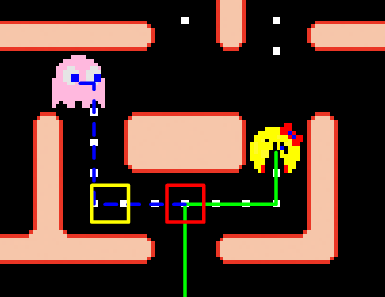
\includegraphics[scale=.3]{closest.png}
\caption{$\mathbf{closest(}\vec{s})$, where $\vec{s}$ is the step marked by the red box, would in this example return the distance between the red and the yellow step.}
\label{fig:closest}
\end{figure}

$D(\vec{s}, \vec{g})$ is computationally the most expensive part of $Q_{\mathrm{step}}$ as it has to calculate the shortest path to each ghosts and is called for each step of each path.  \\

Using $Q_{\mathrm{path}}$ the controller is able to navigate around the maze using the preferences of its genotype. It is easy to construct a genotype that enables the controller to perform well by intuitively selecting the parameters manually but it is difficult to construct a genome with an optimal combination of values. The goal of applying EA to Pac-Man was to optimize the combination of genotype parameters to create a good controller.

\begin{table}
\begin{center}
\caption{Genotype}
\label{table-genotype}
\begin{tabular}{|l|c|}
\hline
Variable    & Range	\\
\hline
$g_{pill}$ & $-1,000$ - $1,000$\\
\hline
$g_{multiplier}$ & $-10$ - $10$\\
\hline
$g_{power}$ & $-1,000$ - $1,000$\\
\hline
$g_{ghost}$ & $-10,000$ - $10,000$\\
\hline
$g_{death}$ & $-10,000$ - $10,000$\\
\hline
$g_{win}$ & $-10,000$ - $10,000$\\
\hline
$g_{step}$ & $-1,000$ - $1,000$\\
\hline
$g_{danger}$ & $0$ - $100$\\
\hline
$g_{kill}$ & $0$ - $100$\\
\hline
\end{tabular}
\end{center}
\end{table}

One could argue that allowing a negative value for eating pills is unnecessary as it would only produce bad controllers but by allowing a wide range of values, both positive and negative, more strategies will be tested and maybe a strategy not foreseen is shown to perform well. When generating a random genotype all the parameters are given a random value within their respective range (see Table \ref{table-genotype}).

Uniform crossover was selected in the implemented EA as the reproduction strategy since no clear relationship between the genotype parameters was identified. The fitness function simply plays the game a number of times with the phenotype against the Legacy ghosts and returns the average score. 

\subsection{Parameters and performance}
Due to the high amount of path finding calculations in the implemented controller it will take a long time to run just one generation and it was thus necessary to select parameters that enabled the EA to reach a satisfying result within a reasonable amount of time. A rather small population of only 20 genotypes was selected as it minimizes the running time while still being able to have some variation in the gene pool. The mutation rate (the chance for an offspring to mutate) is set to 80\% to spread the search fast in the relative few generations the EA will produce. A mutation strategy is selected that for each parameter, in a genotype hit by mutation, changes it at a 11\% chance to a new randomized value within its range. With this mutation strategy some mutated genotypes will undergo several changes while others will be left unchanged. To increase the spread in the search space crossover always happen in contrast to some techniques that uses a crossover probability \cite{GAsurvey}. The fitness function uses the average of only three play-throughs also to minimize the running time with the cost of being imprecise and the change of killing unlucky, but fit, genotypes. 

\begin{figure}[!htb]
\centering
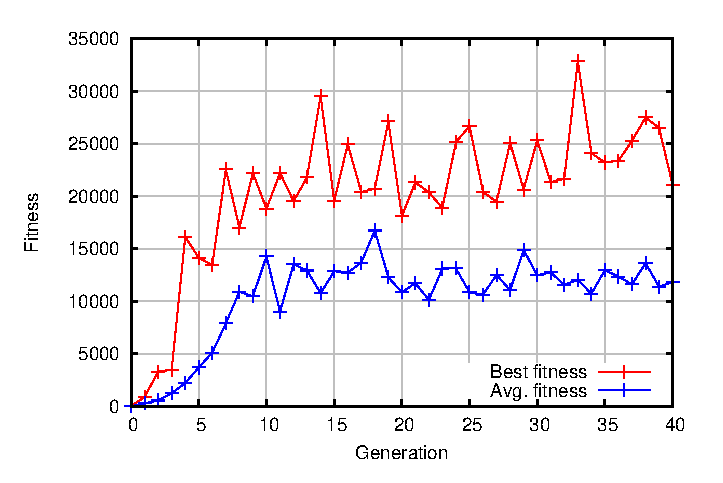
\includegraphics[scale=.7]{ga.eps}
\caption{Best and average fitness of population through 40 generation.}
\label{fig:EABF}
\end{figure}

It took approximately 60 hours to run the implemented EA 40 generations using the described parameters on a modern PC. The evolution of 40 generations was not reproduced due to the long running time. The population reaches fitness scores between 18,000 and 33,000 after only eight generations where the curve begins to plateau. The best and average fitness scores of each generation can bee seen on Figure~\ref{fig:EABF}. It is noticeable that after the 8th generation the fitness scores oscillates. From generation 33 to 34 the best fitness score drops from 32,853 to 24,123 even though the genotype that produced the high score of 32,853 in generation 33 still remained (unaltered) in generation 34. It can thus be concluded that using only three play-throughs in the fitness function gives very imprecise fitness scores. The most fit genotype of the 40th generation can be seen in Table \ref{fig:EABF}.\\

\begin{table}
\begin{center}
\caption{Best genotype found}
\label{table-best-genotype}
\begin{tabular}{|l|c|}
\hline
Variable    		& Value	\\
\hline
$g_{pill}$ 			& 473\\
\hline
$g_{multiplier}$ 	& 3.19\\
\hline
$g_{power}$ 		& 688\\
\hline
$g_{ghost}$ 		& 9,768\\
\hline
$g_{death}$ 		& -8,513\\
\hline
$g_{win}$ 			& 3,055\\
\hline
$g_{step}$ 			& 521\\
\hline
$g_{danger}$ 		& 79\\
\hline
$g_{kill}$ 			& 4\\
\hline
\end{tabular}
\end{center}
\end{table}

The best genotype from the 40th generation were played against three different ghost controllers. The minimum, maximum and average scores from 40 play-throughs together with the sample standard deviation using Bessels's correction can be seen on Table \ref{GAscores}.

\begin{table}
\begin{center}
\caption{The scores of 40 play-throughs. }
\label{GAscores}
\begin{tabular}{|l|c|c|c|c|}
\hline
Ghost controller & Min. & Max. & Avg. & Deviation \\
\hline
Aggressive & 7,260 & 23,840 & 16,330 & 4,246\\
\hline
Legacy & 3,720 & 36,010 & 16,006 & 7,474\\
\hline
Legacy2 The Reckoning & 3,720 & 32,920 & 12,621 & 6,329\\
\hline
\end{tabular}
\end{center}
\end{table}

\subsection{Experiments}
Notice the sudden rise of the fitness score at generation 3 on Figure \ref{fig:EABF}. It looks like a genotype has been created with far better fitness value than the best from the previous generation. The GA was run for 10 generations three times to see some the different results. The plots can be seen in the Appendix and shows some fairly different progressions but all with a steady growth in fitness.

\subsection{Conclusions}
The implemented GA was able to find a solution with a satisfying result. The best solution found reached an average score of 16,006 against the Legacy ghosts and a maximum of 36,010 points. The implemented GA was run with a population of 20 genotypes and ran until the 40th generation was reached which took approximately 60 hours, but a satisfying solution with a fitness score of above 20,000 was found already in the 7th generation. The GA was run three additional times until the 10th generation and all runs reached a best fitness score above 15,000. The fitness function used returns the average of only three play-throughs and produced very inconsistent values meaning the best fitness score found in a generation is usually higher than the actual best fitness score. 

\subsection{Discussion}
The average scores reached by the best solution in the 40th generation are lower than it could be expected to be when looking at Figure \ref{fig:EABF}. The high scores reached by the best solution in each generation seems to be reached simply because the number of potential solutions in the population is high and it only takes one solution to play three good games in a row to reach a high fitness score. I believe the reason why the evolution stops where is does simply is the limit of the design of the phenotype and the genotype and this would be the part I would revisit it I were find a better solution using GA in Pac-Man.  

\section{Monte-Carlo Tree Search}
While the goal of Evolutionary Algorithms is to find an optimal solution, such as the best parameters for a Pac-Man controller, Monte-Carlo Tree Search (MCTS) tries to find the best decision in a given state much like the MiniMax algorithm. MiniMax has been implemented in a lot of deterministic games with perfect information with success, such as in Chess and Checkers, but it requires an approximate evaluation function \cite{ShannonChess} when it does not have time to search all the way to terminal states. In games with huge branching factors and/or imprecise evaulation functions the MiniMax algorithm usally fails \cite{MCTSframework} but the MCTS has shown to be successful in some of these games, such as GO \cite{MCTSsurvey}.\\

MCTS is a best first search that use random sampling as a heuristic instead of en evaluation function. It builds up a tree with the root node holding the current game state. A node can for each possible action in its state be expanded to have a child node with the resulting state, just as in the MiniMax algorithm. MCTS has the following four steps that are executed sequentially until its time budget is reached:

\begin{enumerate}
  \item \emph{Selection:} A tree policy is applied to the tree to recursively select the most urgent child node until an expandable and non-terminal node is reached.
  \item \emph{Expansion:} The selected node is expanded (expansions can either be full or partial).
  \item \emph{Playout}: A game is played from the selected node to a terminal state using the default policy. Also called rollouts or simulations. 
  \item \emph{Backpropagation:} The outcome of the playout is backpropagated to the root node where each node has its value and visit count updated.
\end{enumerate}

The default policy can simply be a random playout but better results can often be achieved by adding domain knowledge \cite{MCTSsurvey}. The tree policy should balance the search between exploitation and exploration and to do this the Upper Confidence bounds applied to Trees (UCT) is used.

\begin{align}
UCT=\overline{X}_{j}+C_{p}\sqrt{\frac{2 \ln n}{n_{j}}} \nonumber
\end{align}

where $n$ is the visit count of the current node, $n_{j}$ is the visit count of the child $j$, $C_{p}$ is a constant determining the amount of exploration over exploitation and $\overline{X}_{j}$ is the normalized value of child $j$ \cite{MCTSsurvey}. In the selection step the child with the highest UCT value is the most urgent and will be selected over its siblings.

\subsection{Approach}
The approach for the MCTS implementation in this paper uses some of the ideas described by T. Pepels and M. Winands \cite{MCTS-Pac-Man} but with some differences. 
The branching factor in Pac-Man in quite small as she can move in only four directions at each step in the game and ghosts can only change direction in junctions. The game tree is however very deep with up to 24,000 ticks in the game as Pac-Man can change direction at each tick. The MCTS do not need to form a search tree with a depth of 24,000 but it is critical that it least reaches the next junction which can be more than 40 steps away. To take this into account an abstraction is used that only accepts game states where Pac-Man is dead, is in a junction, has reached the next level or if the maximum game time is reached. Pepels and Winands use the same abstraction but I treat turns as junctions as well where a turn is a step with two possible non-opposite neighbors. Additionally, reverse moves for Pac-Man is only considered in the first ply to reduce the search tree just as Pepels and Winands do. \\

An important alteration that was implemented, also inspired by Pepels and Winands, was the time limited tree depth (in ticks). 
Expansions in the tree are made by simulating how the Aggressive ghost controller moves and by moving Pac-Man the same direction until a junction is reached (or is in any of the other accepted states). The Aggressive ghost controller were used as they are deterministic and a path will thus not be rated good or bad due to luck. This can however turn out to be a problem if the controller plays against another ghost controller that not always moves aggressively against Pac-Man.
Pepels and Winands also implemented three strategies that changed how the best move was selected but this was not implemented in my controller. 

\subsection{Parameters and performance}
An encoder was implemented that can encode the search tree into XML to make it easier to study. Using the data in the XML I have made a graph representation of the search tree on top of the game graphics (see Figure \ref{fig:MCTSPac-Man}) and a tree representation (see Figure \ref{fig:MCTStree}) of the same situation. The XML output can be seen in the Appendix. 

\begin{figure}[!htb]
\centering
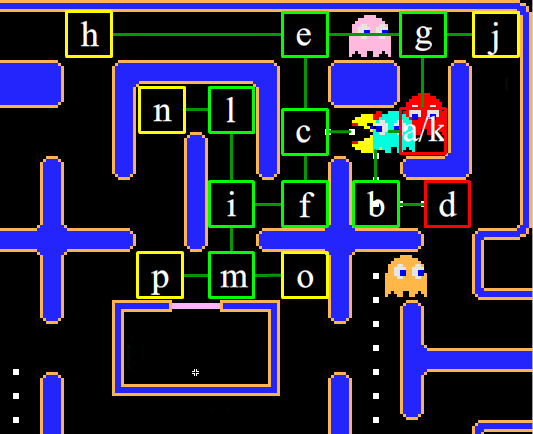
\includegraphics[scale=.3]{mcts-pacman.png}
\caption{A graph representation of the search tree on top of the game graphics. Terminal nodes appear red and nodes deeper than 55 ticks are yellow.}
\label{fig:MCTSPac-Man}
\end{figure}

\begin{figure}[!htb]
\centering
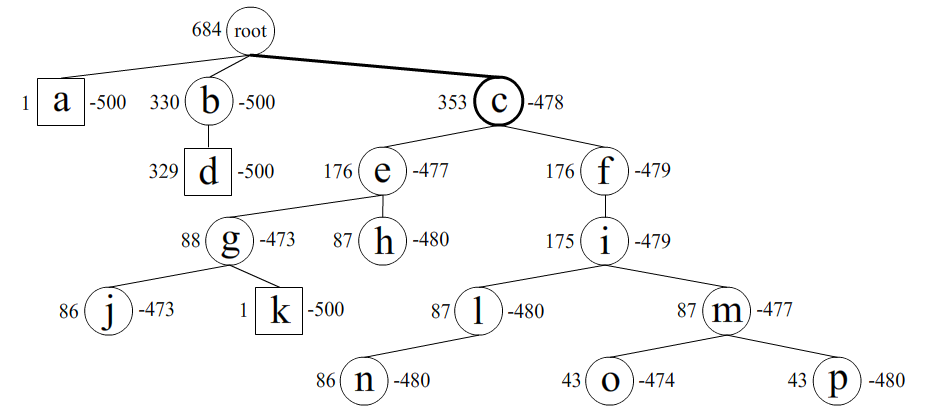
\includegraphics[scale=.28]{mcts-tree.png}
\caption{A tree representation of the same situation as on Figure  \ref{fig:MCTSPac-Man} with the visit count on the left of each node and its average reward on the right. Action $c$ was selected.}
\label{fig:MCTStree}
\end{figure}

The reward of a rollout is the difference between the score of the root node and the score achieved by the rollout. If Pac-Man dies during a rollout -500 is added to the reward. The maximum tree depth is set to 55 ticks and the UCT constant $C=1.5$ which is the same used by Pepels and Winands but I achieve better results by setting the maximum time for rollouts to 200 ticks where Pepels and Winands use only 80 ticks. 

\begin{table}
\begin{center}
\caption{The scores of 40 play-throughs 
with a calculation limit of 40 ms. per tick. }
\label{MCTSscores}
\begin{tabular}{|l|c|c|c|c|}
\hline
Ghost controller & Min. & Max. & Avg. & Deviation \\
\hline
Aggressive & 116,300 & 155,920 & 137,120 & 8,114 \\
\hline
Legacy & 14,790 & 98,750 & 51,523 & 22,422 \\
\hline
Legacy2 The Reckoning & 7,910 & 66,660 & 30,816 & 12,671 \\
\hline
\end{tabular}
\end{center}
\end{table}

\subsection{Experiments}
Two experiments with the MCTS algorithm have been made. The first experiment tests the algorithm with harder time constraints than normal and shows that the algorithm still performs acceptable with a calculation time of only 8 ms. per move (see Table \ref{MCTSscorestime}). 

The seconds experiment tests the algorithm while it uses a random ghost controller in the default policy to see if it can achieve better against the Legacy2 ghosts. The tests shows the algorithm performs slightly worse against both Legacy and Legacy2 (see Table \ref{MCTSscoresRollout}). Additionally, Legacy2 was applied to the rollouts which produced a slightly better result against Legacy2.

\begin{table}
\begin{center}
\caption{The scores of 40 play-throughs with a lower calculation time than normally required. All games are played against the Legacy ghost controller. }
\label{MCTSscorestime}
\begin{tabular}{|l|c|c|c|c|}
\hline
Calculations time & Min. & Max. & Avg. & Deviation \\
\hline
8 ms. & 7,980 & 78,440 & 35,221 & 15,979\\
\hline
4 ms. & 5,720 & 60,610 & 26,869 & 12,178 \\
\hline
2 ms. & 6,380 & 34,460 & 19,847 & 8,182 \\
\hline
\hline
40 ms. & 14,790 & 98,750 & 51,522 & 22,422 \\
\hline
\end{tabular}
\end{center}
\end{table}

\begin{table}
\begin{center}
\caption{The scores of 10 play-throughs with another ghost controller used in rollouts. Calculation time of 40 ms. }
\label{MCTSscoresRollout}
\begin{tabular}{|l|l|c|c|c|c|}
\hline
Ghost contr. & Rollout & Min. & Max. & Avg. & Deviation \\
\hline
Legacy & Random & 27,360 & 62,240 & 42,323 & 10,601\\
\hline
Legacy2 & Random & 14,780 & 39,610 & 24,360 & 7,689 \\
\hline
Legacy2 & Legacy2 & 23,700 & 54,790 & 38,081 & 8,540 \\
\hline
\end{tabular}
\end{center}
\end{table}


\subsection{Conclusions}
The MCTS was able to achieve very good scores against all of the three ghost controllers used in the test. The algorithm uses the Aggressive ghost controller when expanding the tree and the Legacy ghost controller during rollouts. The algorithm achieved an average score of 137,120 against the Aggressive ghost controller and an average score of 51,523 against Legacy. The algorithm struggled a bit more against Legacy2 with an average of 30,816 but when Legacy2 was applied to the rollouts the algorithm performed slightly better with an average score of 38,081 (second average calculated from 10 games only). The scores are a lot lower than the avarage of 107,561 (against Legacy2) that T. Pepels and M. Winands \cite{MCTS-Pac-Man} reached using MCTS, but their implementation relied heavily on their strategy enhancement which is a feature I did not implement. Pepels and Winands reached an average score of 44,758 when they disabled their strategy enhancement which is not that far from my results.

\subsection{Discussion}
Using a specific ghost controller in the tree expansion and in the rollouts makes the algorithm better against those controllers than against other controllers. By using random ghosts in the rollouts the algorithm becomes less biased and I hoped it would also improve. It did play a lot safer by using random rollouts but it also became unable to exploit the weaknesses of the enemy. A difficult choice when applying MCTS to Pac-Man seems to be the balance between exploitation of known ghost strategies and playing safe against a wide range of ghosts. Pepels and Winands most important enhancement seems to be their strategy enhancement which would be the key point of interest if I were to improve the MTCS controller.

\section{Reinforcment lLearning}
Reinforcement Learning (RL) is a family of techniques used to train an agent to know which actions are the most rewarding in given situations. The training is a simple trial and error process where the agent learns by interacting with the environment. Using RL in Pac-Man the agent should learn which move is most rewarding at each possible state of the game. The Markov Property says that transitions and rewards only depend upon the current state and the current action, even if the transition and rewards are probabilistic \cite{RLthesis}. 
Q-learning is a RL technique which uses temporal difference learning by calculating and updating the quality of a transition. A so-called Q-table is used to store the quality value for each action possible in each state. When a new state $s_{t\mathrm{+1}}$ is reached by performing $a_{t}$ in $s_{t}$ the following quality function is used to calculate the new quality value for $a_{t}$ in $s_{t}$:

\begin{eqnarray}
Q_{t\mathrm{+1}}(s_{t}, a_{t}) = (1-\alpha) \, Q_{t}(s_{t}, a_{t}) + \nonumber \\  
\alpha \, \Big(R_{t\mathrm{+1}} + \gamma \, \underset{a} {max} \, Q_{t} (s_{t\mathrm{+1}},a)\Big) \nonumber 
\end{eqnarray}
where $\alpha$ is the learning rate between 0 and 1, $R_{t\mathrm{+1}}$ is the reward of reaching the new state $s_{t\mathrm{+1}}$, $\gamma$ is the discount factor between 0 and 1 that rates rewards in the near future higher than rewards in the far future and $Q_{t} (s_{t\mathrm{+1}},a)$ is the previous quality of $a_{t}$ in $s_{t}$. 

The critical part in Reinforcement learning is the modeling of states. If the modeled states do not capture the relevant information needed to predict the reward the agent cannot learn the optimal decision, but if the modeled states are too complex the state space will be too large to learn.

\subsection{Approach}
The state space in Pac-Man is large. Just taking into account the hundreds of possible positions for Pac-Man and the ghosts gives us billions of permutations ($100^{5}=10,000,000,000$) and it is thus necessary to make an abstract representation of the game state. I have decided only to focus on the first level of the game to simplify the problem. The game state abstraction for this implementation (see Table \ref{abgamestate}) has $64 \times 4^{4} \times 2^{8} = 4,194,304$ permutations which was only possible as pills are ignored. Since Pac-Mans position is narrowed down only to junctions and turns the controller will only be able to change direction in these.

\begin{table}
\begin{center}
\caption{The game state abstraction. }
\label{abgamestate}
\begin{tabular}{|l|l|l|}
\hline
Variable & Description \\
\hline
$s_{\mathrm{junction}} \in \mathbb{N}$ & Junction/turn Pac-Man is in. \texttildelow 64 per level.\\
\hline
$s_{\mathrm{up}} \in \left\lbrace 1,4,16,64 \right\rbrace$ & Distance to ghost by moving up. \\
\hline
$s_{\mathrm{right}} \in \left\lbrace 1,4,16,64 \right\rbrace$ & Distance to ghost by moving right. \\
\hline
$s_{\mathrm{down}} \in \left\lbrace 1,4,16,64 \right\rbrace$ & Distance to ghost by moving down. \\
\hline
$s_{\mathrm{left}} \in \left\lbrace 1,4,16,64 \right\rbrace$ & Distance to ghost bymoving left. \\
\hline
$s_{\mathrm{edibleup}} \in \left\lbrace 0,1 \right\rbrace$ & Is ghost by moving up edible? \\
\hline
$s_{\mathrm{edibleright}} \in \left\lbrace 0,1 \right\rbrace$ & Is ghost by moving right edible? \\
\hline
$s_{\mathrm{edibledown}} \in \left\lbrace 0,1 \right\rbrace$ & Is ghost by moving down edible? \\
\hline
$s_{\mathrm{edibleleft}} \in \left\lbrace 0,1 \right\rbrace$ & Is ghost by moving left edible? \\
\hline
$s_{\mathrm{tlpp}} \in \left\lbrace 0,1 \right\rbrace$ & Is top left power pill still in the level? \\
\hline
$s_{\mathrm{trpp}} \in \left\lbrace 0,1 \right\rbrace$ & Is top right power pill still in the level? \\
\hline
$s_{\mathrm{blpp}} \in \left\lbrace 0,1 \right\rbrace$ & Is bottom left power pill still in the level? \\
\hline
$s_{\mathrm{brpp}} \in \left\lbrace 0,1 \right\rbrace$ & Is bottom right power pill still in the level? \\
\hline
\end{tabular}
\end{center}
\end{table}

\subsection{Parameters and performance}
The learning rate $\alpha$ was set to 0.2, the discount factor $\gamma$ to 0.9 and the exploitation rate used in the training was set to 0.7.

When training the controller it both learns fast and slow. Fast because after only 76,500 runs it is able to score around 5,000 points and slow because the number of learned states after 4,916,500 runs (it took approx. 9 hours on a modern PC) only reached a number of 22,527 which is only 0.537\% of the entire state space. When watching the trained controller play it is often able to get all the power pills before it runs out of lives, and for each power pill eaten is also able to eat a couple of ghosts.

\begin{figure}[!htb]
\centering
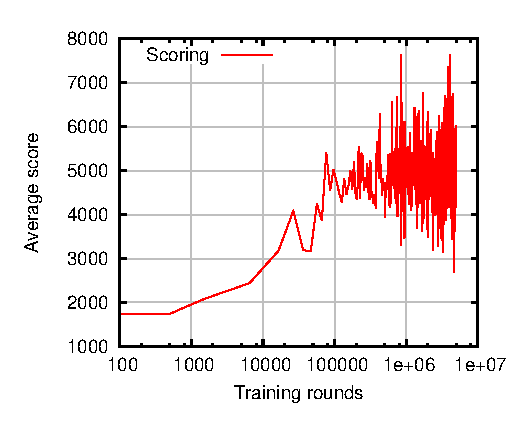
\includegraphics[scale=.7]{qstdscore}
\caption{The average scoring of 5 games for the controller after a number of training rounds.}
\label{fig:Qscore}
\end{figure}

\subsection{Experiments}
An experiment was performed in which the exploitation factor was changed to a new random number between 0 and 1 every 1000th run to see if the controller would learn faster. In the experiment, which was not reproduced, 16,852 states where reached in 976,500 runs in contrast to the 2,246,500 runs required previously which is 230\% faster, but the number of states learned after 976,500 runs was only 117\% higher. The growth in learned states can be seen on Figure \ref{fig:Qstates}.

\begin{figure}[!htb]
\centering
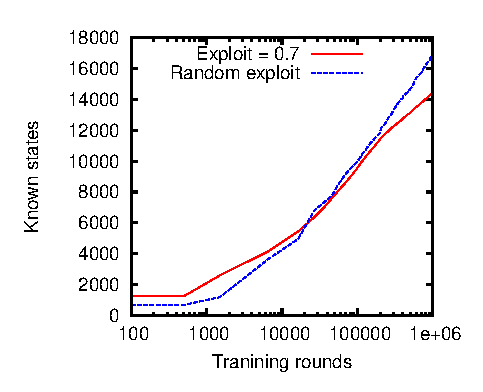
\includegraphics[scale=.7]{states-tl}
\caption{The number of known states during training.}
\label{fig:Qstates}
\end{figure}

\subsection{Conclusions}
The implemented Q-learning algorithm was able to train a Pac-Man controller to play the first level in the game with a score of around 5,000 points before running out of lives. The algorithm only learned 0.537\% of the state space in 4,916,500 runs which very slow. 
An experiment with a variable randomized learning rate showed to speed up the learning process by 230\% but it was only able to find 117\% more states after 976,500 runs as the number of states found over times decreases gradually. The Q-learning algorithm thus seem to be to slow to learn more than just a couple percent of the state space.

\subsection{Discussion}
Even though the controllers performance was not terrible compared to my expectations, it seems the state space designed is to large to learn within a reasonably amount of time. To decrease the size of the state space even further I would suggest using a higher level of abstraction, e.g. by removing the junction variable from the state representation and replace it by a junction type variable which e.g. could be a left turn or an intersection with four directions. The variable type would then have 9 different values. A new problem would however appear as the position of Pac-Man relative to a power pill is not captured. It would probably be necessary also to remove the power pill booleans and replace them by a distance variable like with the ghosts but then the state space would grow to a size of $9\times4^{8}\times2^{4}=9,437,184$. I have not been able to find a state representation which has a smaller state space while it still captures the important details. By looking back at the implemented state representation it has a clear problem when eating ghosts as it only knows whether the closest ghost is edible and thus a non-edible ghost could thus appear right behind the edible one, so it seems the state representation i first designed does not capture all the required details.

\begin{thebibliography}{3}

\bibitem{Pac-Mancompetition}
\emph{Ms. Pac-Man Competition, screen-capture}. \hskip 1em plus 0.5em minus 0.4em\relax
 http://www.Pac-Man-vs-ghosts.net/, accessed October, 2013.

\bibitem{EC}
A. E. ~Eiben and J. E. Smith  \emph{Introduction to Evolutionary Computing}.\hskip 1em plus 0.5em minus 0.4em\relax
  Springer, 2003, pp. 19--21.
  
\bibitem{GAsurvey}
M. ~Srinivas and L. M. Patnaik  \emph{Genetic Algorithms: A Survey}.\hskip 1em plus 0.5em minus 0.4em\relax
  Motorola India Electron. Ltd., 1994, pp. 1--8.

\bibitem{ShannonChess}
C. E. ~Shannon  \emph{Programming a Computer for Playing Chess}.\hskip 1em plus 0.5em minus 0.4em\relax
  Bell Telephone Laboratories, Inc., 1949, pp. 1--7.

\bibitem{MCTSframework}
G. ~Chaslot, S. ~Bakkes, I. ~Szita and P. ~Spronck  \emph{Monte-Carlo Tree Search: A New Framework for Game AI}.\hskip 1em plus 0.5em minus 0.4em\relax
  Universiteit Maastricht, 2008/10.

\bibitem{MCTSsurvey}
C. ~Browne, E. ~Powley, D. ~Whitehouse, S. ~Lucas, P. I. ~Cowling, P. ~Rohlfshagen, S. ~Tevener, D. ~Perez, S. ~Samothrakis and S. ~Colton  \emph{A Survey of Monte Carlo Tree Search Methods}.\hskip 1em plus 0.5em minus 0.4em\relax
  IEEE Transactions on computational intelligence and AI in games, vol. 4, no. 1, March 2012, pp. 1-22.

\bibitem{MCTS-Pac-Man}
T. ~Pepels and M. H.M. ~Winands  \emph{Enhancements for Monte-Carlo Tree Search in Ms Pac-Man, PhD thesis}.\hskip 1em plus 0.5em minus 0.4em\relax
  IEEE Conference on Computational Intelligence and Games, 2012.

\bibitem{RLthesis}
C. J.C.H. ~Watkins.  \emph{Learning from Delayed Rewards, PhD thesis}.\hskip 1em plus 0.5em minus 0.4em\relax
  King' College, 1989, pp. 37-53.


\end{thebibliography}

\pagebreak

\section{Appendix}

\begin{figure}[!htb]
\centering
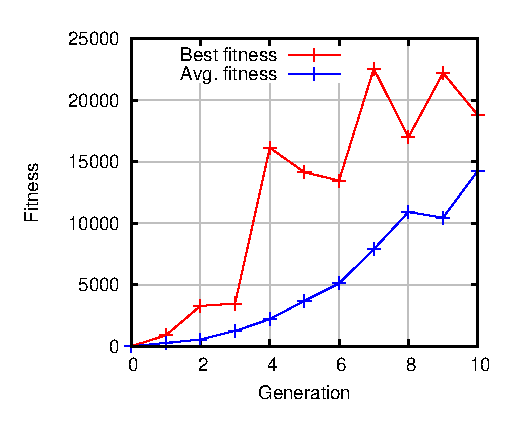
\includegraphics[scale=.7]{gashort0.eps}
\caption{First 10 generations of Figure \ref{fig:EABF}.}
\label{fig:EASHORTA}
\end{figure}

\begin{figure}[!htb]
\centering
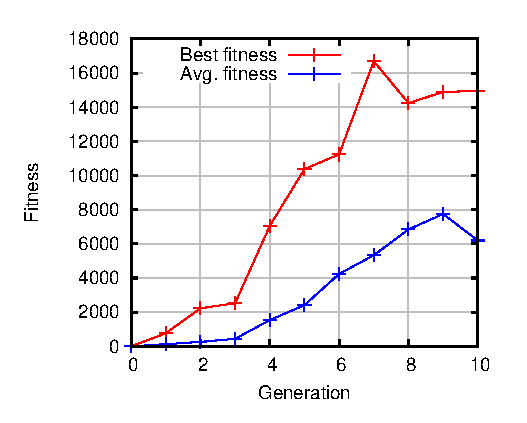
\includegraphics[scale=.7]{gashorta.eps}
\caption{Best and average fitness of population through 10 generations.}
\label{fig:EASHORTA}
\end{figure}

\begin{figure}[!htb]
\centering
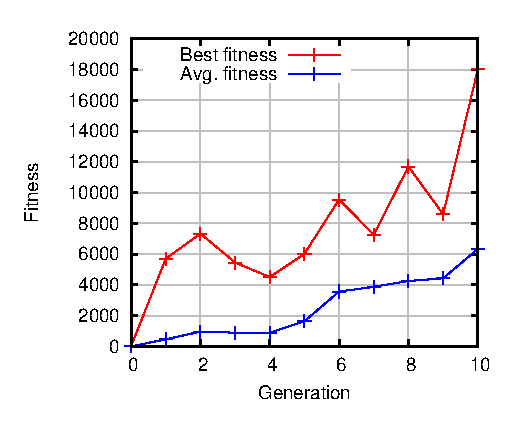
\includegraphics[scale=.7]{gashortb.eps}
\caption{Best and average fitness of population through 10 generations.}
\label{fig:EASHORTB}
\end{figure}

\begin{figure}[!htb]
\centering
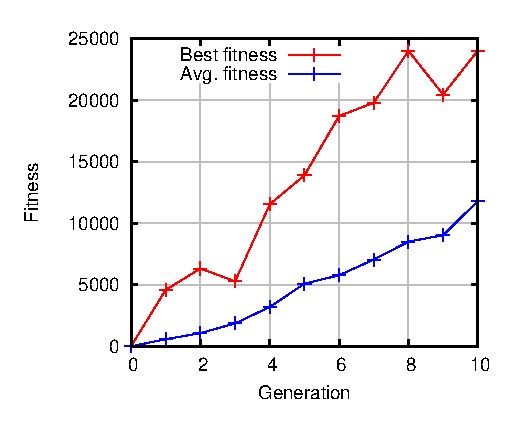
\includegraphics[scale=.7]{gashortc.eps}
\caption{Best and average fitness of population through 10 generations.}
\label{fig:EASHORTC}
\end{figure}

\begin{figure}[!htb]
\centering
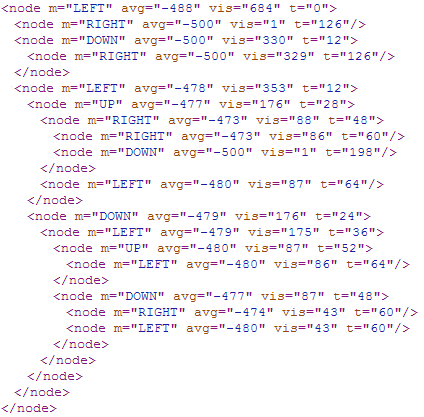
\includegraphics[scale=.6]{xml.png}
\caption{The search tree of Figure \ref{fig:MCTStree} encoded in XML.}
\label{fig:EASHORTC}
\end{figure}

\begin{figure}[!htb]
\centering
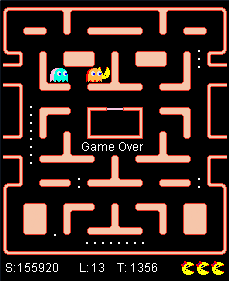
\includegraphics[scale=.6]{155920.png}
\caption{The high score of 155,920 points reached by the MCTS controller against the Aggressive ghost controller.}
\label{fig:MCTShighscore}
\end{figure}

\end{document}
